\documentclass[conference]{assets/latex/IEEEtran}

\usepackage{amsmath,amssymb,amsfonts}
\usepackage{graphicx}

\graphicspath{{assets/latex/}}

\begin{document}

\title{CS6524 Computer Vision Lab.~2\\
Camera Calibration and Stereo Vision}

\author{
\IEEEauthorblockN{James Kelly}
\IEEEauthorblockA{
23370858\\
Immersive Software Engineering\\
University of Limerick, Ireland
}
\and
\IEEEauthorblockN{Aaron Roche}
\IEEEauthorblockA{
[Student ID]\\
Immersive Software Engineering\\
University of Limerick, Ireland
}
\and
\IEEEauthorblockN{James Doherty}
\IEEEauthorblockA{
[Student ID]\\
Immersive Software Engineering\\
University of Limerick, Ireland
}
}

\maketitle

\section{Introduction}

This lab investigates camera calibration and depth estimation
using videos recorded on phone cameras. Checkerboard images
are used to estimate camera intrinsics and lens distortion.
Pairs of scene frames are then used to estimate camera motion
and generate depth maps. Coloured point clouds are exported
from selected depth frames to visualise the reconstructed scene.


\section{Methodology}

\subsection{Video Preparation}

Calibration videos were recorded using each member's phone.
The checkerboard was mounted on a rigid surface to reduce
warping, and different views of the board were captured.
Separate scene videos were recorded using sideways camera
movement around stationary objects at different depths.

Twenty calibration frames were selected by dividing
checkerboard detections into temporal bins and choosing
the sharpest frame in each bin using Laplacian variance.
This spread the selected frames throughout the recording
rather than taking several similar neighbouring frames.


\subsection{Corner Detection}

Each calibration frame was converted to grayscale before
detecting corners with \texttt{cv2.findChessboardCorners}.
The printed board contained $9\times6$ squares, giving
an $8\times5$ inner-corner grid. The detector was configured
to match this board rather than the $9\times6$ inner-corner
dimensions stated in the brief.

Detected corners were refined using
\texttt{cv2.cornerSubPix} to obtain sub-pixel coordinates.
These image points were passed to the calibration stage
with their corresponding checkerboard object points.
Figure~\ref{fig:corners} shows an example detection.

\begin{figure}[!t]
    \centering
    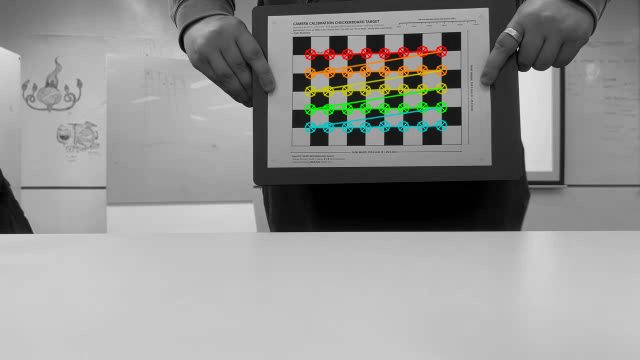
\includegraphics[
        width=0.75\columnwidth
    ]{calib_corners.png}
    \caption{Detected $8\times5$ inner-corner grid for
    camera 01. The board was mounted on a rigid surface.}
    \label{fig:corners}
\end{figure}

% Add the group's remaining methodology here.


\subsection{Point-Cloud Export}

One depth frame per scene was exported as a coloured
PLY point cloud. The exporter selects the frame pair
with the most valid depth values within 250~cm.

The depth values and camera parameters were used to
calculate the 3D position of each retained pixel.
Colours were taken from the corresponding image
and saved alongside the point coordinates.

Invalid depths and points beyond 250~cm were excluded.
If no frame pair contains valid points, the program
reports a warning instead of exporting an empty cloud.


\section{Discussion and Failure Analysis}

% To be completed with the group's final results and analysis.

\end{document}